
\subsection{Iteración 1}

Durante esta iteración se van a diseñar todas las pruebas que habrá en el proyecto. Se ha elegido que haya tres pruebas de cada tipo para mostrar suficiente variedad en ellas, pero que no sean una cantidad demasiado grande para este proyecto.


\subsubsection{Pruebas de motricidad}




Para cada prueba de baile es necesario elegir una canción y tres pasos. Un paso puede ser una posición concreta de las extremidades, un movimiento concreto entre dos puntos de una extremidad, o también puede ser un momento de libertad en el que el usuario pueda moverse según le plazca al ritmo de la música. En esta prueba se busca estimular el movimiento y flexibilidad del usuario, así como su coordinación. Los momentos de libertad no solo permiten estimular estas capacidades si no que también actuan de vía de expresión para los sentimientos y estado del jugador. Es importante elegir música con la que los mayores estén familiarizados para hacer que se sientan inmersos y cómodos con la canción y el baile. Teniendo todo esto en cuenta se han elejido las siguientes tres canciones junto a sus pasos:

\begin{itemize}
    
    \item {Ejemplo 1: El chacachá del tren – El consorcio
    \begin{itemize}
        \item {Brazos arriba y abajo alternados}
        \item {Libre}
        \item {Brazos arriba y abajo alternados}
    \end{itemize}}
    
    \item {Ejemplo 2: Las flechas del amor – Karina
    \begin{itemize}
        \item {Brazo izquierdo de izquierda a derecha}
        \item {Brazo derecho de izquierda a derecha}
        \item {Libre}
    \end{itemize}}
    
    \item {Ejemplo 3: Chica ye-ye – Concha Velasco
    \begin{itemize}
        \item {Brazos arriba y abajo alternados}
        \item {Ambos brazos a la izquierda y derecha a la vez}
        \item {Libre}
    \end{itemize}}

\end{itemize}

La siguiente prueba de motricidad es la de figuras, que consiste en que el jugador adopte tres poses concretas de forma encadenada. Para que el jugador tenga tiempo de colocarse en posición, habrá cinco segundos de margen entre cada cambio de posición. Para definir un ejemplo de este tipo de prueba es necesario escoger un conjunto de tres poses corporales. Los tres ejemplos escogidos son:
	
\begin{itemize}
    	
    \item {Ejemplo 1: 
    \begin{itemize}
        \item {Ambos brazos arriba}
        \item {Brazo izquierdo abajo, derecho a la derecha}
        \item {Ambos brazos al frente}
    \end{itemize}}
    \item {Ejemplo 2:
    \begin{itemize}
        \item {Brazo derecho al frente, izquierdo arriba}
        \item {Brazo derecho en diagonal abajo, izquierdo en diagonal arriba}
        \item {Ambos brazos arriba}
    \end{itemize}}
    \item {Ejemplo 3:
    \begin{itemize}
        \item {Ambos brazos en diagonal abajo}
        \item {Ambos brazos al frente}
        \item {Ambos brazos en diagonal arriba}
    \end{itemize}}

\end{itemize}

Para la última prueba de motricidad, la de parada, el jugador tiene que repetir un movimiento de forma constante y cuando sea necesario parar en seco y mantener la posición. Con esta prueba se estimula aún más la movilidad del jugador además de su tiempo de reacción. En este caso solo es necesario definir el movimiento que el jugador seguirá, ya que el momento en el que tendrá que parar se decidirá aleatoriamente en cada prueba con un intervalo de entre 10 y 15 segundos.


\begin{itemize}
    \item {Ejemplo 1: Mover los brazos de arriba abajo al contrario (brazo derecho arriba mientras el izquierdo está abajo)}
    \item {Ejemplo 2: Trazar círculos en el frente con cada una de las manos}
    \item {Ejemplo 3: Trazar un círculo con la mano derecha mientras se sube y baja la izquierda.}
\end{itemize}


\subsubsection{Pruebas de memoria}


En las pruebas de memoria se intenta estimular la memoria a largo plazo del jugador. En la prueba de turismo se estimula la memoria mediante imágenes icónicas de diferentes ciudades y monumentos famosos a nivel mundial. La imagen se muestra en la pantalla principal del escenario del concurso y el jugador tiene que describirla, recordar su nombre, su localización y todo lo que sea capaz de recordar. Para esta prueba se han elegido las siguientes tres imágenes: 

\begin{itemize}
    \item {Ejemplo 1: Torre Eiffel, París, Francia. Figura \ref{fig:E4_torreEiffel}}
    \item {Ejemplo 2: Coliseo, Roma, Italia. Figura \ref{fig:E4_coliseo}}
    \item {Ejemplo 3: Estatua de la libertad, Nueva York, EE. UU. Figura \ref{fig:E4_estatuaLibertad}}
\end{itemize}




\begin{figure}[H]
\centering
\begin{minipage}{.3\textwidth}
  \centering
  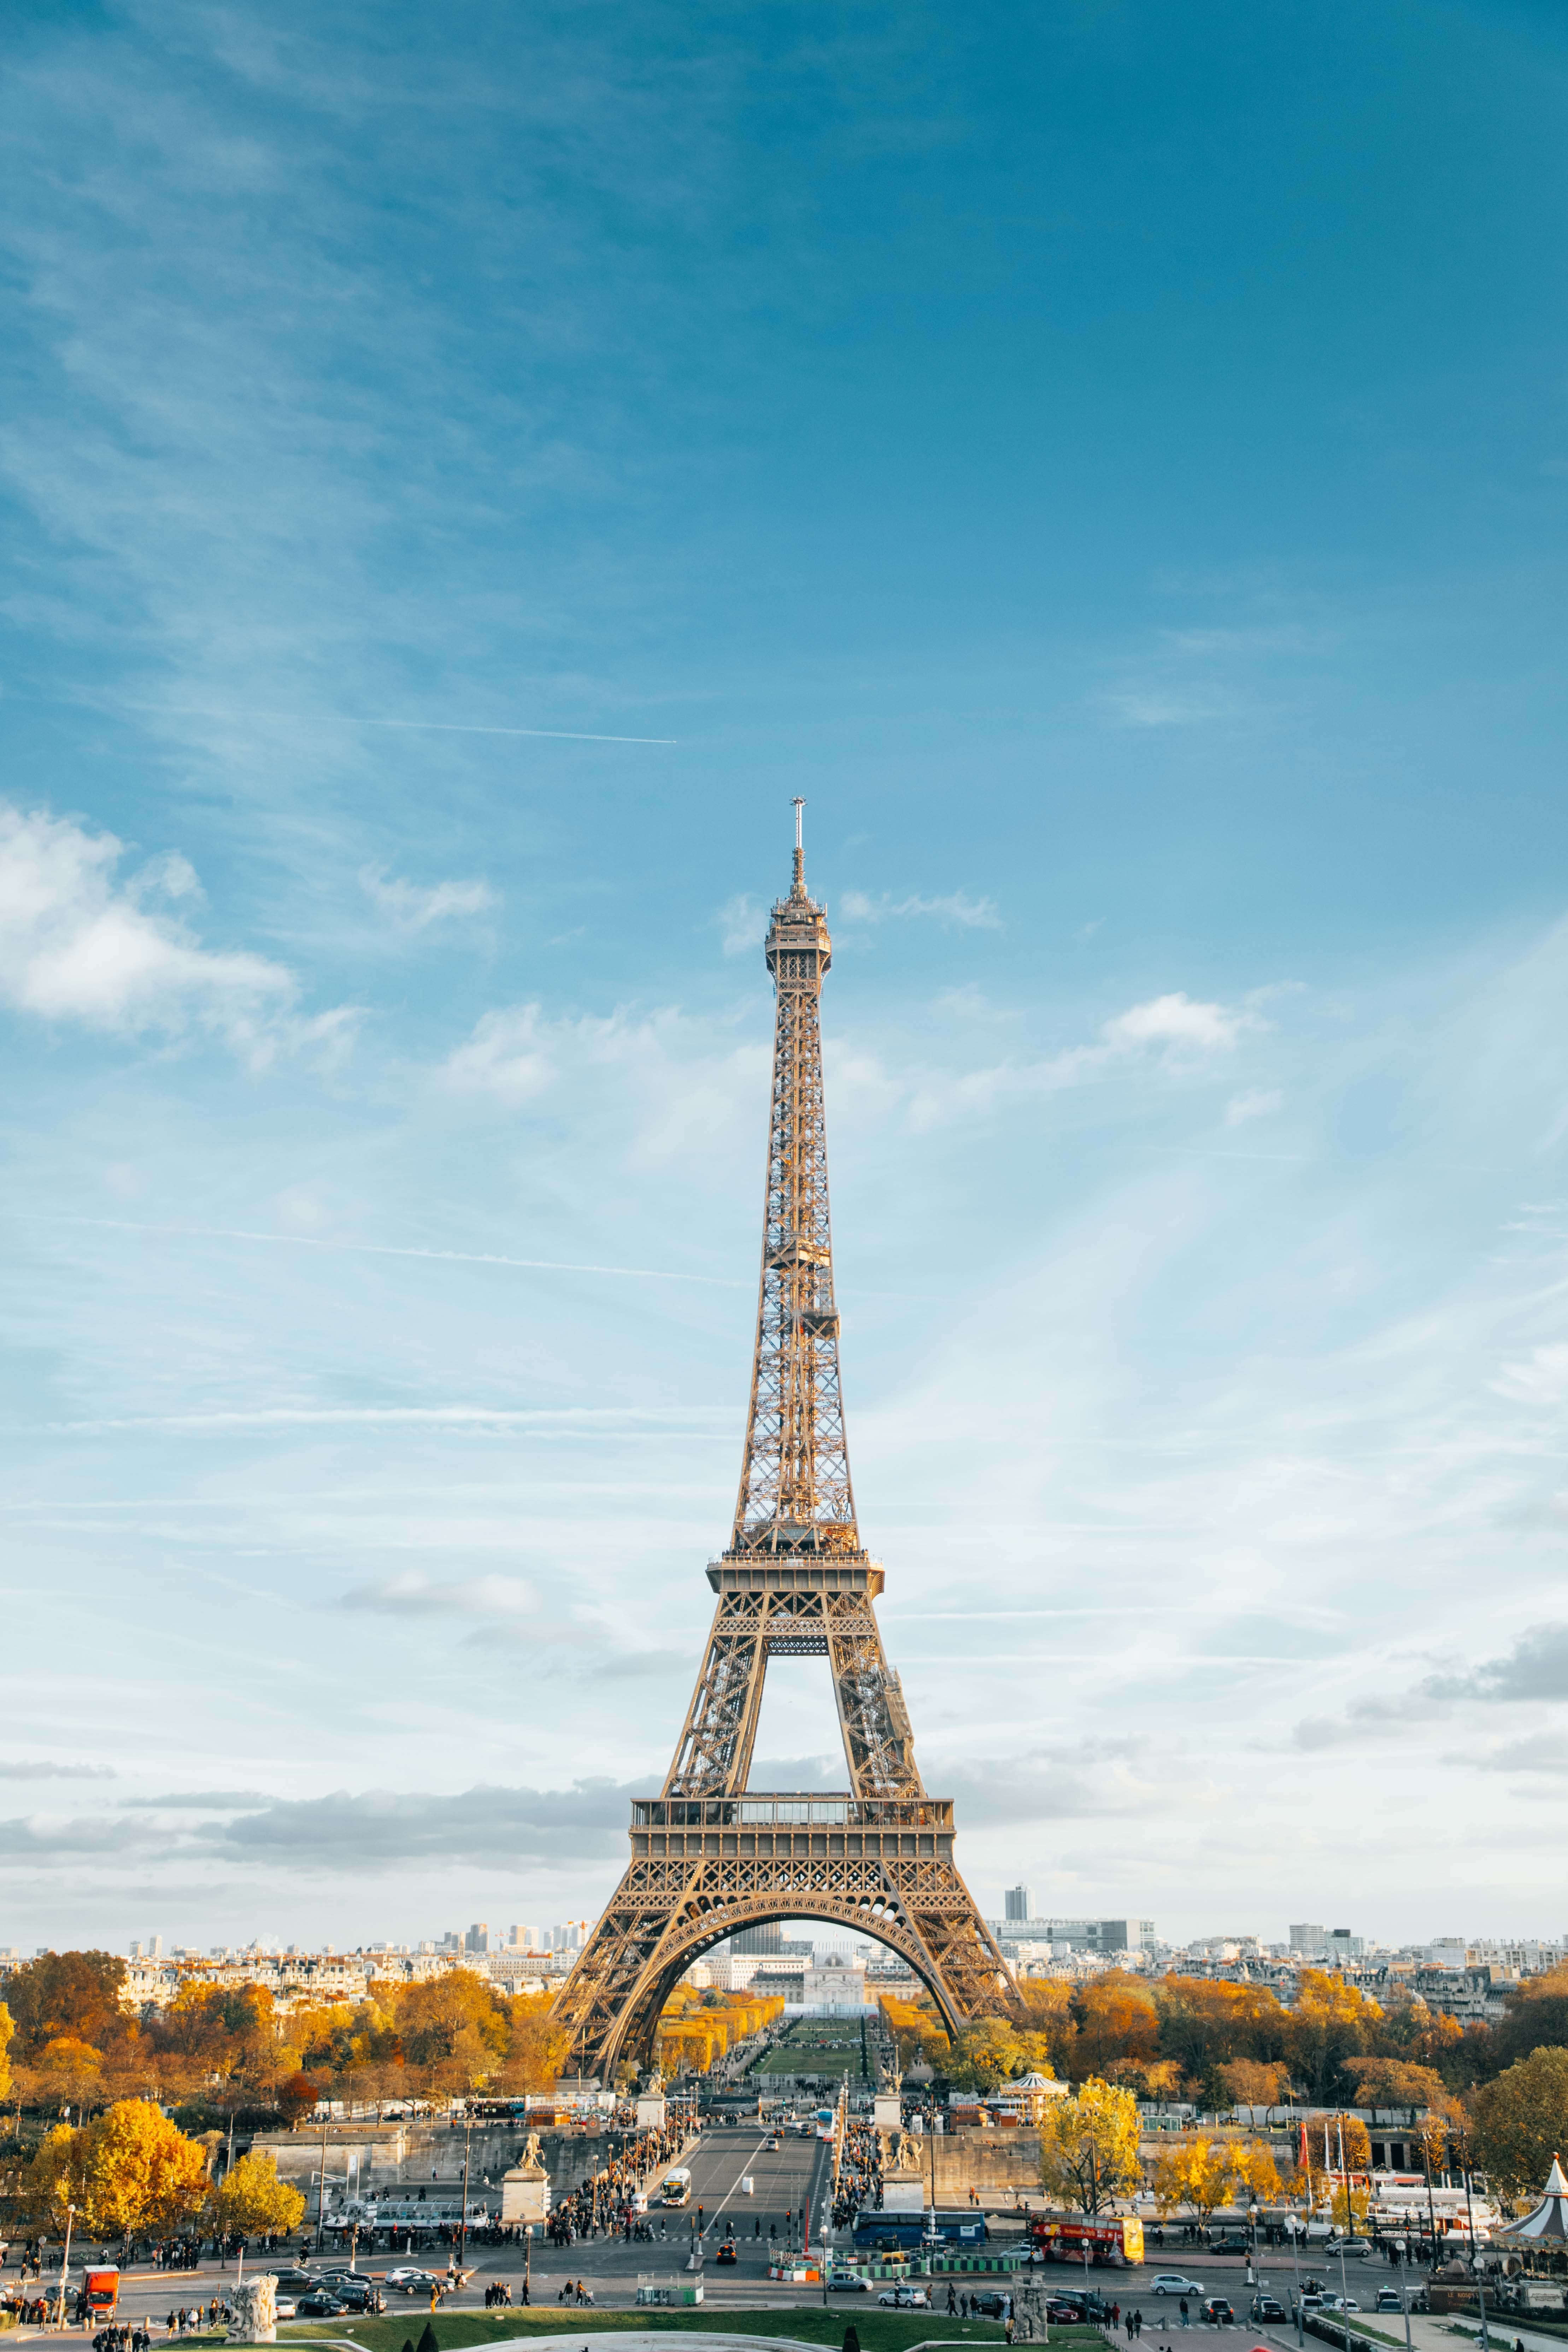
\includegraphics[width=.7\linewidth]{04.Desarrollo/04.Entrega4/01.Iteracion4_1/00.Figuras/01.eiffel.jpg}
  \captionof{figure}{Torre Eiffel, París, Francia.}
  \label{fig:E4_torreEiffel}
\end{minipage}%
\begin{minipage}{.3\textwidth}
  \centering
  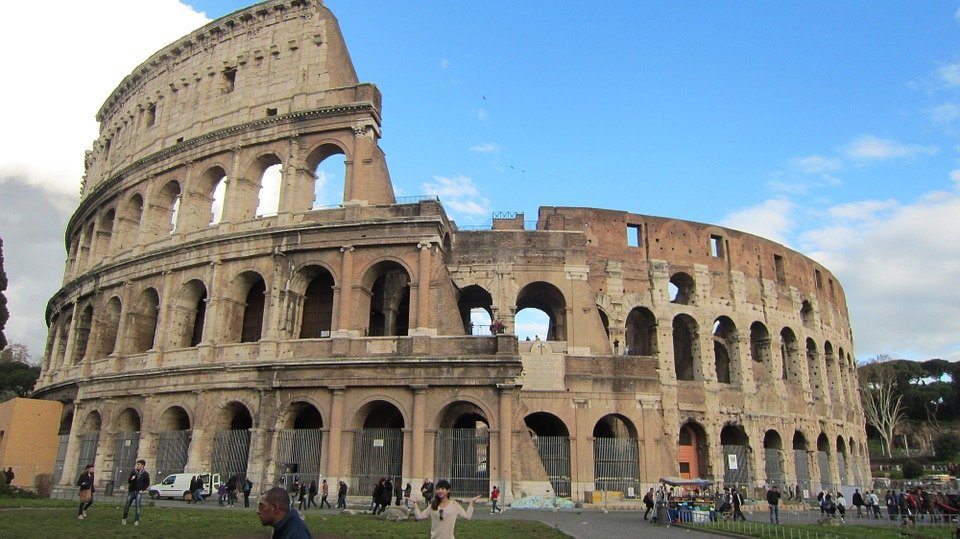
\includegraphics[width=.9\linewidth]{04.Desarrollo/04.Entrega4/01.Iteracion4_1/00.Figuras/02.coliseo.jpg}
  \captionof{figure}{Coliseo romano, Roma, Italia.}
  \label{fig:E4_coliseo}
\end{minipage}
\begin{minipage}{.3\textwidth}
  \centering
  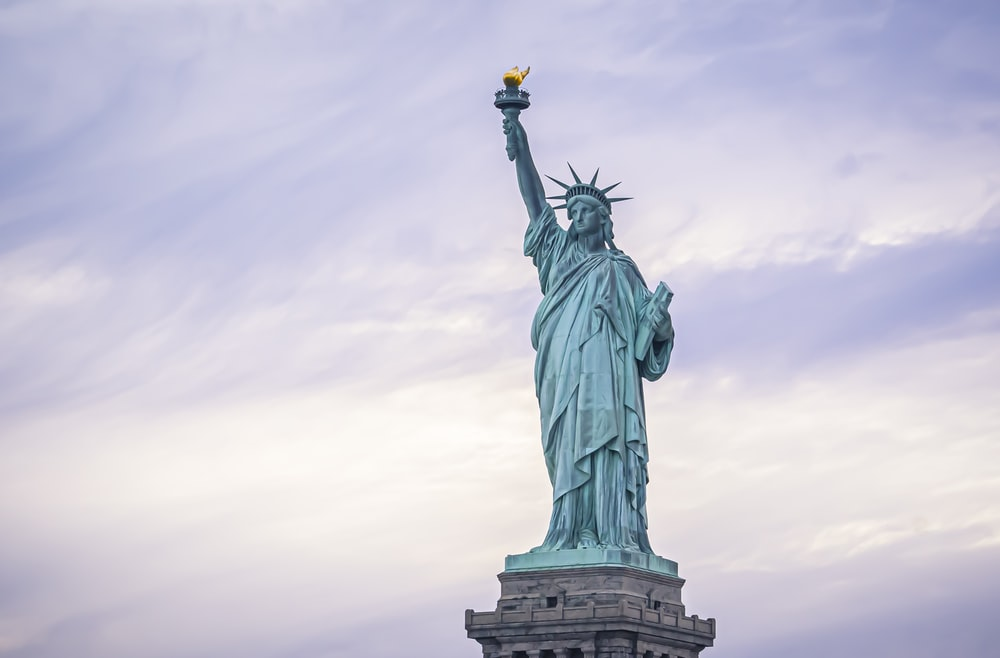
\includegraphics[width=.9\linewidth]{04.Desarrollo/04.Entrega4/01.Iteracion4_1/00.Figuras/03.libertad.jpg}
  \captionof{figure}{Estatua de la libertad, Nueva York, EE. UU.}
  \label{fig:E4_estatuaLibertad}
\end{minipage}
\end{figure}



La prueba de adivinar la canción utiliza el sentido del oído para despertar recuerdos y sentimientos del jugador, por esto es necesario utilizar canciones que sean reconocibles y agradables para las personas mayores cuando estén jugando. En este caso se usarán las siguientes canciones en español:

\begin{itemize}
    \item {Ejemplo 1: Dos gardenias – Antonio Machín}
    \item {Ejemplo 2: Que viva España – Manolo Escobar}
    \item {Ejemplo 3: La luna enamorada – Los Bocheros}
\end{itemize}

\subsubsection{Prueba de lenguaje}

En la prueba de situaciones se intenta que el jugador razone y hable sobre una situación concreta. Para ello se mostrará una imagen en la pantalla del escenario que representará una situación concreta. Se intenta que el jugador esté inmerso en la experiencia y pueda desarrollar sus pensamientos sobre la imagen, por lo que es importante que se traten de situaciones comunes, por las que probablemente hayan pasado y que les evoque sentimientos. Se han elegido estas imágenes:

\begin{itemize}
    \item {Ejemplo 1: Médico vendando la mano de una persona. Figura \ref{fig:E4_medico}}
    \item {Ejemplo 2: Madre preparando a su hijo para el colegio. Figura \ref{fig:E4_colegio}}
    \item {Ejemplo 3: Gente bailando en la Feria de Abril. Figura \ref{fig:E4_feria}}
\end{itemize}



\begin{figure}[H]
\centering
\begin{minipage}{.3\textwidth}
  \centering
  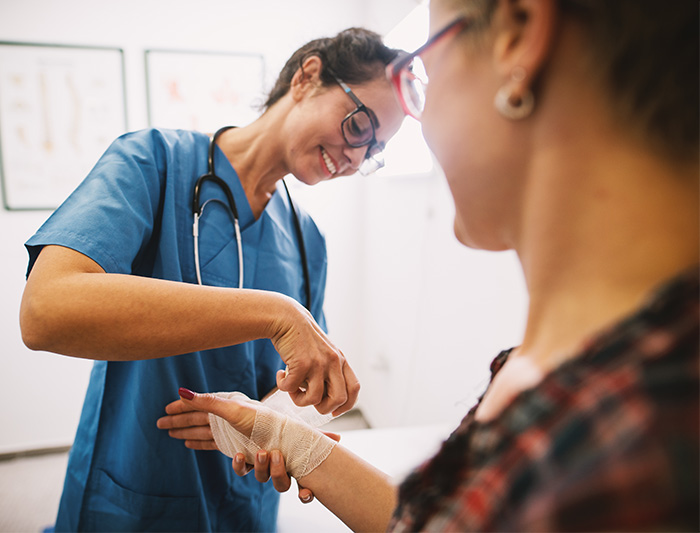
\includegraphics[width=.9\linewidth]{04.Desarrollo/04.Entrega4/01.Iteracion4_1/00.Figuras/04.medico.jpg}
  \captionof{figure}{Médico vendando una mano.}
  \label{fig:E4_medico}
\end{minipage}%
\begin{minipage}{.3\textwidth}
  \centering
  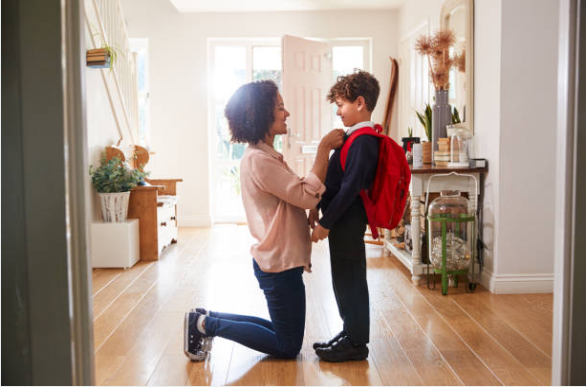
\includegraphics[width=.9\linewidth]{04.Desarrollo/04.Entrega4/01.Iteracion4_1/00.Figuras/05.colegio.png}
  \captionof{figure}{Madre preparando a su hijo para el colegio.}
  \label{fig:E4_colegio}
\end{minipage}
\begin{minipage}{.3\textwidth}
  \centering
  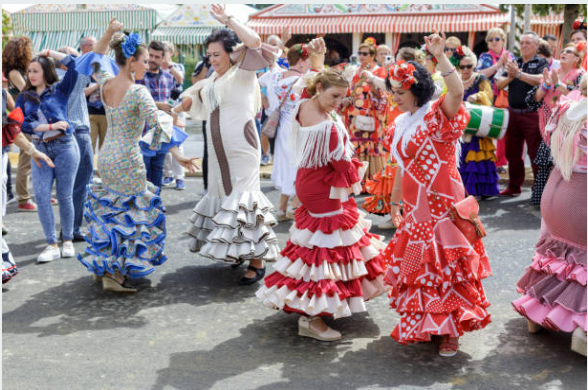
\includegraphics[width=.9\linewidth]{04.Desarrollo/04.Entrega4/01.Iteracion4_1/00.Figuras/06.feria.png}
  \captionof{figure}{Gente bailando en la feria de abril.}
  \label{fig:E4_feria}
\end{minipage}
\end{figure}


\subsubsection{Pruebas de razonamiento}


En estas pruebas se intenta activar y ejercitar el razonamiento del jugador. La prueba de agrupación de objetos intenta que el jugador descubra las dos categorías ocultas en las que se clasifican los objetos que se le muestran. Es necesario que estos objetos sean fácilmente reconocibles en forma de objeto virtual tridimensional, así como claramente distinguible la categoría a la que pertenecen cuando se presentan con el resto de los objetos. Para cada ejemplo se mostrarán cuatro objetos de dos categorías sobre la mesa del escenario:

\begin{itemize}
    \item {Ejemplo 1: 
        \begin{itemize}
            \item {Frutas: Manzana, plátano}
            \item {Ropa: Zapato, guante}
        \end{itemize}}
    \item {Ejemplo 2:
        \begin{itemize}
            \item {Transporte: Avión, coche}
            \item {Objetos de casa: Bombilla, teléfono}
        \end{itemize}}
    \item {Ejemplo 3:
        \begin{itemize}
            \item {Plantas: Árbol, flor}
            \item {Música: Guitarra, radio}
        \end{itemize}}
\end{itemize}

En la prueba de asociación de sonidos se muestran objetos sobre la mesa de la misma forma que en la prueba anterior, con la única condición de que estos objetos tienen que poder emitir un sonido característico. En este caso, se pueden usar los mismos objetos para los tres ejemplos y lo que cambiará será qué objeto produce el sonido. Para tener variedad de sonidos distinguibles, se han elegido los siguientes:

\begin{itemize}
    \item {Coche}
    \item {Pájaro}
    \item {Guitarra}
    \item {Teléfono}
\end{itemize}


\subsubsection{Pruebas de comprensión espacial}


En las pruebas de comprensión espacial se intenta evaluar la capacidad del jugador de tener una comprensión firme del espacio que lo rodea así como de los estímulos que recibe de él, principalmente mediante la audición o la visión. La prueba de siluetas presenta al usuario con tres siluetas sombreadas y debe descubrir de qué objetos se trata. Las siluetas irán en conjuntos de tres y podrán o no estar superpuestas. Para no aumentar la complejidad del proyecto, se utilizan modelos ya utilizados en otras pruebas agrupados de la siguiente forma:
	
\begin{itemize}
    \item {Ejemplo 1: Coche, teléfono, árbol.}
    \item {Ejemplo 2: Manzana, bombilla, guante.}
    \item {Ejemplo 3: Zapato, plátano, flor.}
\end{itemize}

Finalmente, la prueba de localización de sonidos consiste en colocar una fuente sonora en el espacio al rededor del usuario. El sonido será una persona hablando, ya que es un estímulo muy habitual en la vida real y las posiciones donde aparecerá se elegirán de forma aleatoria en cualquier punto del escenario fuera del campo visual del jugador.

